\scanpage{53}
% letterhead
\begin{center}
{\sffamily INSTITUTE\\
FOR ADVANCED SCIENTIFIC STUDIES}\\[-0.4ex]
\rule{1.7cm}{0.5pt}
\end{center}

\noindent SGA \textbf{5}\qquad \(\overline{\underline{\mathrm{XIII}}}\)

\figure{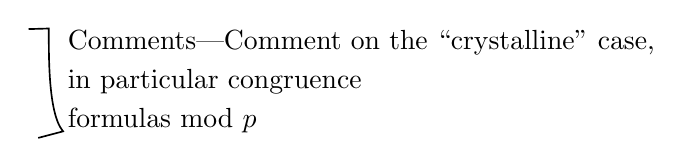
\begin{tikzpicture}
\node[anchor=west,inner sep=0pt,align=left] (lignes) {\unsure{Comments|Comment} on the ``crystalline'' case,\\[0.5ex]
in particular congruence\\[0.5ex]
formulas \(\mathrm{mod}\ p\)};
\draw[semithick] ([xshift=-1.4em,yshift=0.05ex]lignes.north west) --
 ([xshift=-0.67em,yshift=0.10ex]lignes.north west)
 .. controls ([xshift=-0.65em,yshift=-1ex]lignes.north west)
 and ([xshift=-0.75em,yshift=1.8ex]lignes.south west)
 .. ([xshift=-0.15em,yshift=0.20ex]lignes.south west) --
 ([xshift=-1.05em,yshift=-0.35ex]lignes.south west);
\end{tikzpicture}}

\noindent \deleted{\illegible{1}}\quad \(\overline{\underline{\mathrm{IV}}}\)\qquad Pay attention to the relative case, consult \(\overline{\underline{\mathrm{VII}}}\) and SGA 6 \(\overline{\underline{\mathrm{X}}}\)

\noindent \(\overline{\underline{\mathrm{XIV}}}\)\quad (\unsure{Problems|Problems} and \unsure{Comments|Comment})

Mention the variants \(\mathrm{mod}\ p\) and crystalline \unsure{Variants|variants} (cf \unsure{a|my} \unsure{note|notes} on Katz's theorem).
% archive sheet number: 52
\clearpage
